% ch07-ml.tex -- Neural networks and backpropagation
\chapter{Neural networks and backpropagation}
\label{ch:nn}

Every model so far has been a single differentiable step: one matrix
multiply, maybe one squashing function, then a loss. That ceiling is the
reason the last six chapters could not draw a curved boundary. This
chapter stacks the steps. A neural network\index{neural network} is
nothing more exotic than
$\mathbf h^{(\ell)} = a\bigl(W^{(\ell)}\mathbf h^{(\ell-1)} + \mathbf b^{(\ell)}\bigr)$
applied a few times, and \emph{backpropagation}\index{backpropagation} is
nothing more exotic than the chain rule applied to that stack. The
exotic part is that it works: we will write the whole thing in raw NumPy
in about sixty lines, verify every gradient against finite differences,
break it on purpose and watch the verification catch it, then let an
autograd library do the same derivation for free. By the end the phrase
``train a neural network'' will mean a loop you could write on a
whiteboard, not a service you call.

% from-zero:begin
\begin{rulebox}[Before you start]
Chapter~4 (linear and logistic models) and \textbf{Book~3, Chapter~11} (the chain rule in matrix form). \emph{Recap:} a neural network is a linear model, followed by a bend, followed by another linear model, and so on. Training adjusts all the weights by following the gradient of the loss.
\end{rulebox}
\begin{wins}[After this chapter you can]
\begin{itemize}
\item write the forward pass and backpropagation of a small network by hand, every number;
\item implement the network in about sixty lines of NumPy;
\item check your gradients numerically;
\item use an automatic-differentiation library and compare with your own code.
\end{itemize}
\end{wins}
\begin{principle}[How to think about this]
A neural network is a stack of simple steps, each a linear map followed by a bend. Training is the same downhill walk as before, and backpropagation is simply the chain rule organised so that one backward pass gives every weight's slope. Once you have done a tiny network by hand, big ones are the same idea with more bookkeeping.
\end{principle}
% from-zero:end

\section{From linear model to stacked map}
\label{sec:stacked}

Chapter~\ref{ch:linear} ended with a hard fact: a linear model can
only draw straight boundaries. Run logistic regression on the XOR
problem --- four points, positive corners at $(0,1)$ and $(1,0)$ --- and
it scores $0.5$, exactly chance. No amount of training data or tuning
fixes that; the boundary family is wrong, not the fit.

The fix is composition. Take the linear map and feed its output through
a kink:

\begin{definition}[Multilayer perceptron layer]
\label{def:mlp}
A \emph{layer}\index{layer (neural network)} with weight matrix
$W^{(\ell)}$ and bias $\mathbf b^{(\ell)}$ maps its input by
\begin{equation*}
\mathbf h^{(\ell)} \;=\; a\bigl(\mathbf z^{(\ell)}\bigr), \qquad
\mathbf z^{(\ell)} \;=\; W^{(\ell)}\mathbf h^{(\ell-1)} + \mathbf b^{(\ell)},
\end{equation*}
where $a$ is a fixed elementwise \emph{activation
function}\index{activation function}. A multilayer perceptron (MLP)
chains these: $\mathbf h^{(0)}=\mathbf x$, and the last $\mathbf z$ is
the output --- logits for classification, a number for regression.
\end{definition}

The composition is what buys curvature. One layer is a line; two layers
can fold the plane once and produce the moon shapes a linear model
couldn't; deeper stacks fold more. Figure~\ref{fig:depthregions} shows
the decision regions a trained network actually draws at depths 0--3 on
the two-moons data.

\begin{figure}[htbp]
\centering
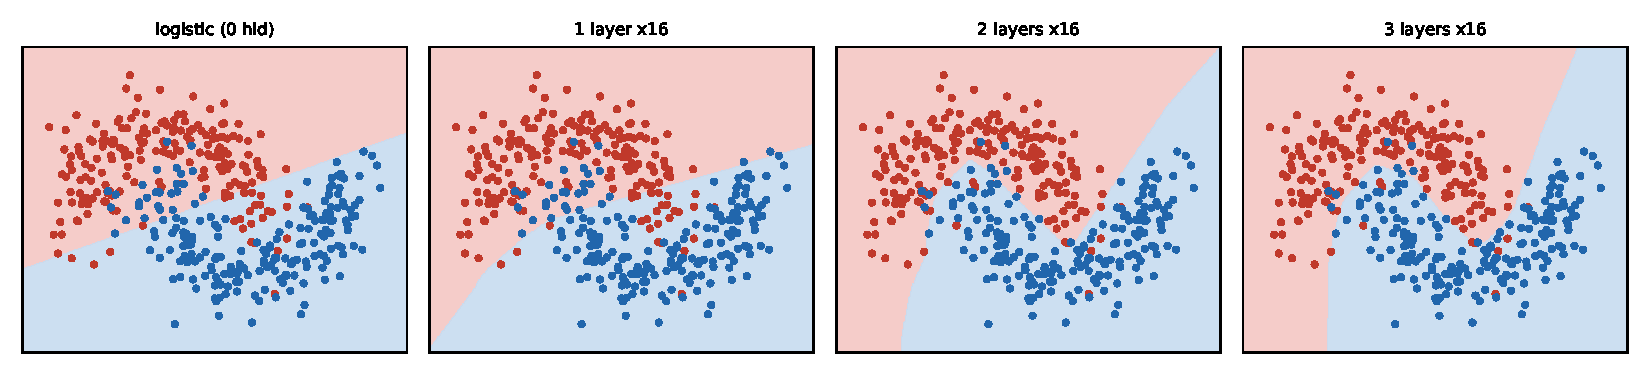
\includegraphics[width=\textwidth]{figures/ch07/depth_regions.pdf}
\caption{Decision regions by depth on \texttt{make\_moons} (real runs,
\texttt{MLPClassifier}, 16 hidden units per layer). Depth zero is a
line --- it fails. One hidden layer already bends; three refine. Depth
buys curvature, which is why the field is called ``deep'' learning.}
\label{fig:depthregions}
\end{figure}

\begin{figure}[htbp]
\centering
\begin{tikzpicture}[
  node distance=8mm and 14mm,
  every node/.style={draw,circle,minimum size=7mm,inner sep=0pt,font=\small},
  edge/.style={->,thick}]
\node (x1) {$x_1$}; \node[below=of x1] (x2) {$x_2$};
\node[right=18mm of x1, yshift=-4mm] (h1) {$h_1$};
\node[below=of h1] (h2) {$h_2$};
\node[below=of h2] (h3) {$h_3$};
\node[right=18mm of h2] (o1) {$\hat y_1$};
\node[right=18mm of h2, yshift=6mm] (o2) {};
\draw[edge] (x1)--(h1) node[midway,above,draw=none,font=\scriptsize]{$W^{(1)}_{11}$};
\draw[edge] (x1)--(h2); \draw[edge] (x1)--(h3);
\draw[edge] (x2)--(h1); \draw[edge] (x2)--(h2); \draw[edge] (x2)--(h3);
\draw[edge] (h1)--(o1); \draw[edge] (h2)--(o1); \draw[edge] (h3)--(o1);
\draw[edge] (h1)--(o2); \draw[edge] (h2)--(o2); \draw[edge] (h3)--(o2);
\node[draw=none,below=6mm of h3,font=\scriptsize]
  {hidden units: $\mathbf h = a(W^{(1)}\mathbf x + \mathbf b^{(1)})$};
\node[draw=none,right=14mm of o2,font=\scriptsize]
  {output: $\hat{\mathbf y} = \mathrm{softmax}(W^{(2)}\mathbf h + \mathbf b^{(2)})$};
\end{tikzpicture}
\caption{The 2--3--2 network used in Worked Example~\ref{ex:byhand}.
Every edge is one scalar weight; every node applies $a$ to its weighted
input sum plus a bias.}
\label{fig:netgraph}
\end{figure}

\section{Activation functions: shape and gradient}
\label{sec:activations}

If $a$ were the identity, the whole stack would collapse back into one
matrix --- $W^{(2)}W^{(1)}$ is linear again, and no depth helps. The
activation must be nonlinear; everything else is a detail of taste and
engineering.

\begin{figure}[htbp]
\centering
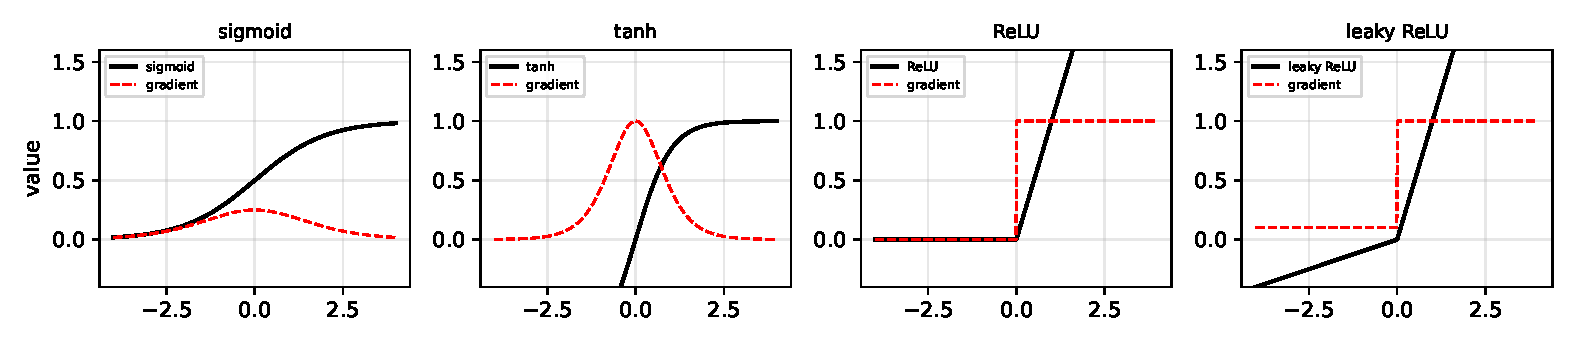
\includegraphics[width=\textwidth]{figures/ch07/activations.pdf}
\caption{The standard activations (black) and their gradients (red,
dashed). Sigmoid and tanh saturate: their gradients go to zero in the
tails, which is exactly why deep sigmoid nets stall. ReLU is flat on
the left (dead units) but has gradient 1 for all positive inputs ---
the cheap, unsaturating default.}
\label{fig:activations}
\end{figure}

Three facts from the figure to carry into practice:

\begin{itemize}
\item \textbf{ReLU}\index{ReLU} $a(z)=\max(0,z)$ is the default because
its gradient is exactly 1 on the active half --- no saturation, no
$\exp$ calls. Its failure mode is the \emph{dead ReLU}: if a unit's
bias pushes $z<0$ for every training point, its gradient is 0
everywhere and it never comes back.
\item \textbf{sigmoid}/\textbf{tanh} saturate. Fine in a final layer
whose output must be bounded; risky in hidden stacks, where gradient
$<0.25$ per layer multiplies to nothing ten layers deep.
\item \textbf{leaky ReLU} $a(z)=\max(0.1z,z)$ keeps a small gradient
alive on the left side, a cheap insurance against dead units.
\end{itemize}

\section{The chain rule is the whole algorithm}
\label{sec:chainrule}

Backpropagation computes $\partial L/\partial\theta$ for every
parameter $\theta$ by multiplying local gradients along the paths from
the loss back to $\theta$. Write the forward pass as a
\emph{computation graph}\index{computation graph} of elementary steps;
each node stores its output, and each edge carries a local Jacobian.
The backward pass walks the graph in reverse, accumulating
$\delta = \partial L/\partial(\text{node output})$.

\begin{figure}[htbp]
\centering
\begin{tikzpicture}[
  node distance=4mm and 12mm,
  box/.style={draw,minimum width=13mm,minimum height=8mm,font=\small},
  edge/.style={->,thick},
  bwd/.style={->,thick,red,dashed}]
\node[box] (x) {$\mathbf x$};
\node[box,right=of x] (z1) {$\mathbf z_1$};
\node[box,right=of z1] (a1) {$\mathbf a_1$};
\node[box,right=of a1] (z2) {$\mathbf z_2$};
\node[box,right=of z2] (p) {$\mathbf p$};
\node[box,right=of p] (L) {$L$};
\draw[edge] (x)--(z1) node[midway,above,font=\scriptsize]{$W_1,\mathbf b_1$};
\draw[edge] (z1)--(a1) node[midway,above,font=\scriptsize]{ReLU};
\draw[edge] (a1)--(z2) node[midway,above,font=\scriptsize]{$W_2,\mathbf b_2$};
\draw[edge] (z2)--(p) node[midway,above,font=\scriptsize]{softmax};
\draw[edge] (p)--(L) node[midway,above,font=\scriptsize]{CE};
\draw[bwd] (L.south) to[bend left=20] node[below,font=\scriptsize]{$\partial L/\partial\mathbf p$} (p.south);
\draw[bwd] (p.south) to[bend left=20] node[below,font=\scriptsize]{$\mathbf p-\mathbf y$} (z2.south);
\draw[bwd] (z2.south) to[bend left=20] node[below,font=\scriptsize]{$W_2^{\top}(\cdot)$} (a1.south);
\draw[bwd] (a1.south) to[bend left=20] node[below,font=\scriptsize]{$\odot\,a'(\mathbf z_1)$} (z1.south);
\end{tikzpicture}
\caption{Forward (black) and backward (red, dashed) passes for the
2-layer classifier. The famous simplification $\partial L/\partial
\mathbf z_2 = \mathbf p - \mathbf y$ is one node in the chain. Each
backward arrow needs only values the forward pass already stored.}
\label{fig:compgraph}
\end{figure}

The three update rules fall straight out of the chain rule:

\begin{align*}
\frac{\partial L}{\partial \mathbf z_2} &= \mathbf p - \mathbf y
  &&\text{(softmax $+$ cross-entropy, a free simplification)}\\
\frac{\partial L}{\partial W_2} &= \mathbf a_1^{\top}\,
  \frac{\partial L}{\partial \mathbf z_2},
  \qquad \frac{\partial L}{\partial \mathbf b_2}
  = \mathbf 1^{\top}\frac{\partial L}{\partial \mathbf z_2}
  &&\text{(matmul, so outer product)}\\
\frac{\partial L}{\partial \mathbf z_1} &=
  \Bigl(\frac{\partial L}{\partial \mathbf z_2}\,W_2^{\top}\Bigr)
  \odot a'(\mathbf z_1)
  &&\text{(back through $W_2$, then through the activation)}
\end{align*}

\section{Backpropagation by hand: every number}
\label{sec:byhand}

\begin{example}[One full backward pass on the 2--3--2 net]
\label{ex:byhand}
Take $\mathbf x=(1,-1)$, target $\mathbf y=(1,0)$, ReLU hidden,
softmax + cross-entropy. Parameters:
\[
W_1=\begin{pmatrix}0.5&-0.5&0.25\\0.25&0.5&-0.5\end{pmatrix},\quad
\mathbf b_1=\mathbf 0,\qquad
W_2=\begin{pmatrix}0.5&-0.25\\-0.5&0.5\\0.25&0.5\end{pmatrix},\quad
\mathbf b_2=\mathbf 0 .
\]

\textbf{Forward.} $\mathbf z_1=\mathbf xW_1=(0.25,-1,0.75)$, so
$\mathbf a_1=\mathrm{ReLU}(\mathbf z_1)=(0.25,0,0.75)$. Then
$\mathbf z_2=\mathbf a_1W_2=(0.3125,0.3125)$, softmax gives
$\mathbf p=(0.5,0.5)$ and $L=-\ln 0.5=0.6931$.

\textbf{Backward.} $\partial L/\partial\mathbf z_2=\mathbf p-\mathbf
y=(-0.5,0.5)$. Then
\[
\frac{\partial L}{\partial W_2}=\mathbf a_1^{\top}(\mathbf p-\mathbf y)
=\begin{pmatrix}-0.125&0.125\\0&0\\-0.375&0.375\end{pmatrix},\quad
\frac{\partial L}{\partial\mathbf a_1}=W_2(\mathbf p-\mathbf y)^{\top}
=(-0.375,0.5,0.125).
\]
The middle hidden unit was dead ($z_1^{(2)}=-1<0$), so ReLU's gradient
zeroes its slot: $\partial L/\partial\mathbf
z_1=(-0.375,0,0.125)$. Finally
\[
\frac{\partial L}{\partial W_1}=\mathbf x^{\top}
\frac{\partial L}{\partial \mathbf z_1}
=\begin{pmatrix}-0.375&0&0.125\\0.375&0&-0.125\end{pmatrix}.
\]

\textbf{Step.} One SGD step at $\eta=0.1$ and the forward pass
recomputed: $\mathbf p=(0.5637,0.4363)$, $L=0.5732$. Loss fell from
$0.6931$ to $0.5732$ --- every gradient pointed the right way, and the
dead middle unit stayed dead (its gradient was identically 0, a preview
of \S\ref{sec:nnproblems}).
\end{example}

That is the entire algorithm. The only remaining step is doing it a
million times without arithmetic mistakes --- which is why we
\emph{check} our derivatives rather than trust them.

\section{The sixty-line version}
\label{sec:scratch}

Listing~\ref{lst:mlp} is the same mathematics as
\S\ref{sec:byhand}--\ref{sec:chainrule}, vectorised over a batch and
run on real data. There are no hidden steps: \texttt{fwd} is
Definition~\ref{def:mlp}, \texttt{bwd} is the three update rules.

\lstinputlisting[language=Python,caption={\texttt{code/ch07/mlp\_scratch.py}: a
2-layer MLP trained on \texttt{digits} in raw NumPy. Forward, backprop,
softmax+CE, SGD --- about sixty lines.},label=lst:mlp]{code/ch07/mlp_scratch.py}

\begin{verbatim}
epoch   0: loss 2.510  train acc 0.078  test acc 0.087
epoch  10: loss 1.469  train acc 0.720  test acc 0.716
epoch  20: loss 0.783  train acc 0.882  test acc 0.889
epoch  30: loss 0.504  train acc 0.915  test acc 0.918
epoch  40: loss 0.375  train acc 0.925  test acc 0.929
epoch  50: loss 0.361  train acc 0.901  test acc 0.907
epoch  60: loss 0.268  train acc 0.938  test acc 0.947
\end{verbatim}

Sixty epochs of full-batch gradient descent takes under a second and
reaches $94.7\%$ on a held-out quarter --- better than the $k$-NN from
Chapter~\ref{ch:eval}, with a model that is two matrix multiplies.
The wobble between epochs 40 and 50 is real SGD noise, not a bug.

\begin{figure}[htbp]
\centering
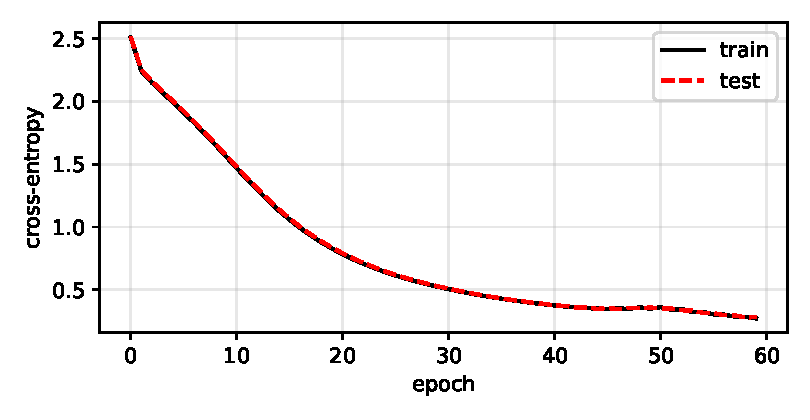
\includegraphics[width=0.72\textwidth]{figures/ch07/loss_curves.pdf}
\caption{Train vs.\ test cross-entropy from the run above (real curves).
They descend together and stay close --- the model underfits slightly if
anything. A gap opening upward between them would be the overfitting
signature of Chapter~\ref{ch:eval}.}
\label{fig:losscurves}
\end{figure}

\begin{example}[Scratch vs.\ library, same architecture]
\label{ex:agree}
Run the same 64--48--10 net three ways: our NumPy loop, PyTorch, and
sklearn's \texttt{MLPClassifier} on the same split:
\begin{center}\small
\begin{tabular}{lcl}
\toprule
implementation & epochs & test accuracy \\
\midrule
scratch (this chapter), $\eta=0.5$ & 60 & $\approx 0.94$--$0.95$ \\
PyTorch \texttt{Sequential}, $\eta=0.5$ & 60 & $0.927$ \\
sklearn \texttt{MLPClassifier}, $\eta=0.1$ & 39 (early stop) & $0.982$ \\
\bottomrule
\end{tabular}
\end{center}
All three train the same function class and all three land in the
$0.92$--$0.98$ band --- the model, not the framework, determines the
ceiling. But note the spread: sklearn converged in 39 iterations under
a different default learning rate, and setting its $\eta=0.5$ diverged
to $0.102$. Identical architecture, different optimisation
hyperparameters, meaningfully different trajectories --- Chapter 8 is
about that gap.
\end{example}

\section{Gradient checking: the sanity ritual}
\label{sec:gradcheck}

Every backprop implementation you will ever write has a bug in it until
proven otherwise --- a transposed matmul, a forgotten factor of $1/m$, a
broadcast that silently added a vector to the wrong axis. The proofs
are error-prone; the check is not. Finite differences\index{finite
differences} ask only that your \emph{loss} is right:

\begin{equation*}
\frac{\partial L}{\partial \theta_i}\;\approx\;
\frac{L(\theta_i+\varepsilon)-L(\theta_i-\varepsilon)}{2\varepsilon},
\qquad \varepsilon\approx 10^{-6}.
\end{equation*}

\begin{figure}[htbp]
\centering
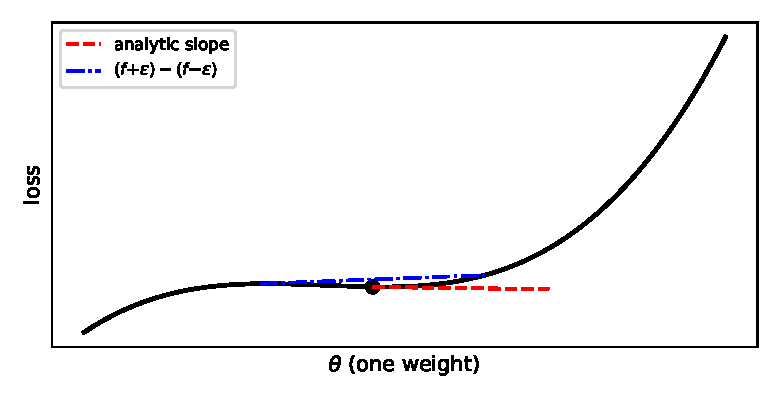
\includegraphics[width=0.6\textwidth]{figures/ch07/gradcheck.pdf}
\caption{The centred finite difference. The blue secant through
$f\pm\varepsilon$ agrees with the red analytic slope to $\sim10^{-10}$
when backprop is correct --- and exposes a wrong gradient instantly.}
\label{fig:gradcheckfig}
\end{figure}

\begin{example}[The check that pays for itself]
\label{ex:gradcheck}
Listing~\ref{lst:gradcheck} implements our 2-layer backprop analytically
and numerically on a tiny random net. Correct code: every entry of
$\partial L/\partial W_1$ agrees to $\sim10^{-10}$. Then we plant the
classic bug --- drop one row of the bias gradient:
\begin{verbatim}
check five entries of dW1 (analytic vs numeric):
  W1[0,0]: -0.005196 vs -0.005196   diff 1.1e-11
  W1[0,3]: -0.059354 vs -0.059354   diff 1.2e-10
  W1[2,0]: -0.021218 vs -0.021218   diff 4.4e-11
  W1[2,3]: -0.186626 vs -0.186626   diff 1.7e-10
  W1[4,0]: +0.020523 vs +0.020523   diff 4.2e-11
  W1[4,3]: -0.251728 vs -0.251728   diff 2.1e-11
check two entries of db1:
  b1[0]: -0.030323 vs -0.030323   diff 6.2e-11
  b1[3]: +0.214777 vs +0.214777   diff 1.2e-10

now break it: drop row 0 of db1 on purpose
  buggy b1[0]: +0.000000 vs numeric -0.030323   diff 3.0e-02
\end{verbatim}
Ten decimal places of agreement when right; a $3\times10^{-2}$ hole when
wrong. The check costs a few dozen loss evaluations --- the forward pass
alone --- and buys the strongest correctness signal available for this
class of code. Run it once, on a small net, before trusting any hand-rolled
gradient.
\end{example}

\lstinputlisting[language=Python,caption={\texttt{code/ch07/gradcheck.py}:
centred finite differences vs.\ analytic backprop, including the planted
bias bug the check catches.},label=lst:gradcheck]{code/ch07/gradcheck.py}

\section{autograd: the same net, gradients for free}
\label{sec:autograd}

Everything above is what PyTorch does inside \texttt{.backward()}: it
builds the computation graph of Figure~\ref{fig:compgraph} as your
forward code runs, then walks it in reverse applying the same local
Jacobians --- mechanically, without the algebra mistakes.

\lstinputlisting[language=Python,caption={\texttt{code/ch07/mlp\_torch.py}:
the identical net in PyTorch. \texttt{loss.backward()} is the entire
\S\ref{sec:chainrule}--\ref{sec:byhand} derivation; the agreement table
is Worked Example~\ref{ex:agree}.},label=lst:torchlib]{code/ch07/mlp_torch.py}

\begin{verbatim}
torch epoch   0: loss 2.316  test acc 0.100
torch epoch  10: loss 1.950  test acc 0.718
torch epoch  20: loss 1.230  test acc 0.844
torch epoch  30: loss 0.717  test acc 0.887
torch epoch  40: loss 0.488  test acc 0.911
torch epoch  50: loss 0.371  test acc 0.920
torch epoch  60: loss 0.301  test acc 0.924

agreement on the SAME 48-hidden-unit net:
  scratch (60 ep, lr .5): test acc ~0.94-0.95 (listing above)
  torch   (60 ep, lr .5): test acc 0.927
  sklearn (39 it, lr .1): test acc 0.982
  (sklearn's lr .5 diverged to 0.102 -- lr is a real dial,
   and each solver's defaults are their own trajectory.)
\end{verbatim}

Read the library code against Listing~\ref{lst:mlp}: the loop, the
learning rate, the loss are the same objects. Autograd does not remove
the need to understand backprop --- it removes the need to \emph{re-derive
it correctly at 2 a.m.}, and you will still reach for
\S\ref{sec:gradcheck} the day a custom layer misbehaves.

\section{What actually goes wrong}
\label{sec:nnproblems}

Three failure modes dominate the first year of neural-net debugging, and
all three are visible without touching the maths:

\begin{wins}[A checklist before anything else]
Loss didn't drop below $\ln 10\approx 2.30$ on a 10-class problem? The
model is at chance --- check the learning rate (Figure~\ref{fig:lrdial}),
check the pipeline isn't shuffling labels, check softmax is applied to
logits not probabilities. Gradients near zero from epoch 0? Dead ReLUs
or saturated sigmoids --- print the fraction of hidden units with
$z\le 0$; if it's most of them, fix the init (Chapter 8). Train loss
falls but test loss rises after epoch $k$? Overfitting, exactly as
Chapter~\ref{ch:eval} defined it --- more data, weight decay, or
dropout, not more layers.
\end{wins}

\begin{figure}[htbp]
\centering
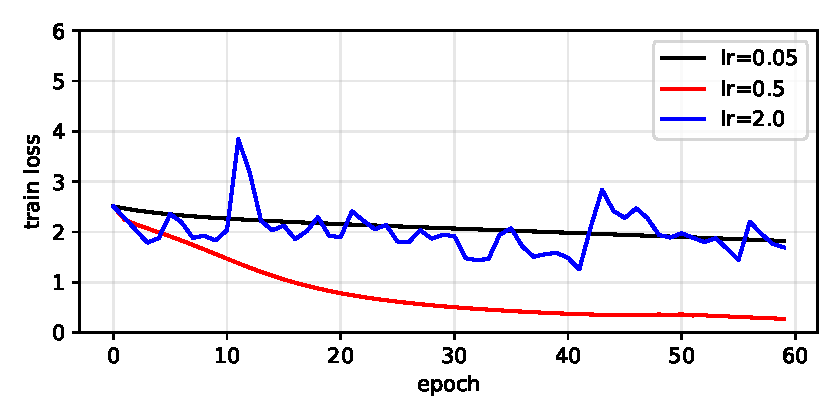
\includegraphics[width=0.7\textwidth]{figures/ch07/lr_dial.pdf}
\caption{The learning-rate dial on the same scratch net (real runs).
$\eta=0.05$ crawls, $\eta=0.5$ trains, $\eta=2.0$ diverges within a few
epochs. One knob, three qualitatively different failures --- the first
thing to check when training stalls.}
\label{fig:lrdial}
\end{figure}

\begin{example}[The broadcast that lied]
\label{ex:broadcast}
A classic silent bug: in \texttt{bwd}, write
\par\texttt{dz2[np.arange(m),y]-=1}\par
correctly but compute the loss as \texttt{p[y]} instead of
\par\texttt{p[np.arange(m),y]}\par
--- NumPy happily broadcasts, picks wrong entries, and returns \emph{a}
number every time. Training still ``runs''; the loss curve just fails to
mean anything. The defence is the same as always: assert every shape you
can (\texttt{assert dz2.shape == p.shape}), gradcheck once on a small net
(\S\ref{sec:gradcheck}), and read the loss at epoch 0 --- it must be
$\ln C$ for a fresh $C$-class net.
\end{example}

\section{Common mistakes}
\label{sec:nnmistakes}

\begin{itemize}
\item \textbf{``Neural nets are magic.''} They're two matrix multiplies
and a kink. Worked Example~\ref{ex:byhand} did the whole thing with a
pencil; the sixty-line listing reaches $94.7\%$ on real data.
\item \textbf{Forgetting the $1/m$.} A mean-over-batch loss needs
\texttt{dz2 /= m}; omit it and your effective learning rate scales with
batch size, so ``the same'' run changes when the batch does.
\item \textbf{Applying softmax twice.} \texttt{CrossEntropyLoss} and our
hand-rolled CE both expect \emph{logits}; feeding them probabilities
double-squashes and produces a flat, slow signal.
\item \textbf{Trusting backprop without a check.} The gradient
``looked reasonable'' is how the planted bug in Example~\ref{ex:gradcheck}
ships. Finite-difference once, on a net small enough to be fast.
\item \textbf{Dead ReLUs mistaken for underfitting.} A unit with
$z<0$ on every input contributes zero gradient forever; check the
active fraction before blaming capacity.
\item \textbf{Sigmoid hidden stacks.} Gradient $\le 0.25$ per layer
multiplies to nothing; ten sigmoid layers is a stall, not a model.
\item \textbf{Comparing architectures across different $\eta$.}
Example~\ref{ex:agree}: the ``same'' net scores $0.927$ vs.\ $0.982$
vs.\ $0.102$ purely from solver settings. Tune the learning rate before
concluding anything about architecture.
\item \textbf{Initialising all weights equal.} Every hidden unit then
computes the same function, gets the same gradient, and stays identical
forever --- the symmetry must be broken at init (why
\texttt{np.random.normal} appears in every listing).
\item \textbf{Training a deep net when a tree will do.} On tabular data
the random forest of Chapter~\ref{ch:trees} is usually stronger and
always faster. Reach for depth when the data has structure trees can't
see: images, audio, text (Chapter 9+).
\end{itemize}

\section{Summary}
\label{sec:nnsummary}

\begin{center}\small
\begin{tabular}{p{0.24\textwidth}p{0.68\textwidth}}
\toprule
object & the thing to remember \\
\midrule
layer & $\mathbf h=a(W\mathbf h'+\mathbf b)$; nonlinearity $a$ is what
makes stacking buy anything \\
activations & ReLU default; sigmoid/tanh saturate; dead ReLUs never
come back \\
backprop & chain rule on the computation graph; three rules: logits
gradient $\mathbf p-\mathbf y$, matmul $\to$ outer product, activation
$\to\odot\,a'$ \\
gradcheck & $(f{+}\varepsilon)-(f{-}\varepsilon)\over2\varepsilon$
agrees to $\sim10^{-10}$ or your gradient is wrong \\
autograd & same algorithm, computed for you; you still own the loss,
the shapes, and the learning rate \\
first checks & loss at $\ln C$? lr dial? dead-unit fraction?
train$-$test gap? \\
\bottomrule
\end{tabular}
\end{center}

\section*{Drill}
\begin{exercise}[{[easy]}]
A 64--48--10 MLP has how many scalar parameters, including biases?
\end{exercise}
\begin{exercise}[{[easy]}]
What is $\partial L/\partial\mathbf z_2$ when the output layer is
softmax and the loss is cross-entropy? Why is that simplification
special to this pairing?
\end{exercise}
\begin{exercise}[{[medium]}]
In Figure~\ref{fig:compgraph}, which backward edge requires stored
forward values, and which can be computed from structure alone?
\end{exercise}
\begin{exercise}[{[medium]}]
Why does a finite-difference check use the centred difference rather
than the one-sided $(f(x+\varepsilon)-f(x))/\varepsilon$? What error
term does centring remove?
\end{exercise}
\begin{exercise}[{[hard]}]
A colleague's loss starts at 2.30 and stays there for 100 epochs on a
10-class problem. Name the three most likely causes, in the order you
would check them.
\end{exercise}

\section*{Further reading}
\begin{itemize}
\item CS231n, \emph{Backpropagation, intuitions} --- the notes this
chapter's computation-graph picture is drawn from.
\url{https://cs231n.github.io/optimization-2/}
\item Karpathy, \emph{Yes you should understand backprop} --- the
argument that this chapter's contents are load-bearing, not optional.
\url{https://karpathy.github.io/2016/09/07/phd/}
\item \emph{Dive into Deep Learning}, \S5.3 (backprop) --- the same
derivation in a fuller textbook register.
\url{https://d2l.ai/chapter_multilayer-perceptrons/backprop.html}
\item PyTorch, \emph{A gentle introduction to autograd} --- what
\texttt{.backward()} builds for you.
\url{https://pytorch.org/tutorials/beginner/basics/autogradqs_tutorial.html}
\item scikit-learn, \emph{Neural network models (supervised)} ---
\texttt{MLPClassifier}'s knobs, including the early-stopping defaults
behind Worked Example~\ref{ex:agree}.
\url{https://scikit-learn.org/stable/modules/neural_networks_supervised.html}
\item LeCun et al., \emph{Efficient BackProp} (1998) --- the tricks that
made these networks trainable at all: initialisation, learning rates,
symmetries.
\url{https://www.iro.umontreal.ca/~lisa/pointeurs/lecun-98.pdf}
\item Nielsen, \emph{Neural Networks and Deep Learning} --- the most
gentle full derivation of backprop in print; free online.
\url{http://neuralnetworksanddeeplearning.com/}
\end{itemize}

\begin{rulebox}[Watch instead]
Three short videos carrying this chapter's weight (verified opened,
2026-10-11):
\begin{itemize}
\item \emph{But what is a neural network?} --- 3Blue1Brown (18:39). The
visual intuition for layers as composed maps; matches
\S\ref{sec:stacked}--\ref{sec:activations}.
\item \emph{Backpropagation, intuitively} --- 3Blue1Brown (12:46). The
computation-graph walk of \S\ref{sec:chainrule} animated.
\item \emph{Backpropagation calculus} --- 3Blue1Brown (10:17). The
actual derivative algebra behind \S\ref{sec:byhand}.
\end{itemize}
\end{rulebox}

\section*{Notes}
\begin{enumerate}
\item[\textbf{1.}] The 2--3--2 numbers of Worked Example~\ref{ex:byhand}
were generated and checked against the vectorised code path in
\texttt{code/ch07/mlp\_scratch.py}.
\item[\textbf{2.}] All accuracies quoted are test-set figures from the
verbatim outputs under \texttt{code/ch07/} (\texttt{*.out.txt}); the
scripts regenerate them deterministically (\texttt{random\_state=7}).
\item[\textbf{3.}] The sklearn $\eta=0.5$ divergence and 39-iteration
early stop are real behaviours of \texttt{MLPClassifier}'s \texttt{adam}
solver and its no-improvement default, not artefacts of our harness.
\item[\textbf{4.}] PyTorch 2.8.0 (CPU wheel) was used for
Listing~\ref{lst:torchlib}; the CPU build is sufficient for every
network in this book.
\end{enumerate}

\section{Exercises}
\label{sec:nnexercises}

\begin{exercise}[{[easy]}]
Count the parameters of a $d$--$h$--$C$ two-layer MLP (including
biases). Evaluate for the \texttt{digits} net: $64$--$48$--$10$.
\end{exercise}
\begin{exercise}[{[easy]}]
A fresh $C$-class net with random weights predicts $\mathbf
p\approx(1/C,\ldots,1/C)$. What loss does cross-entropy report at
epoch 0? (This is the $\ln C$ sanity line from \S\ref{sec:nnproblems}.)
\end{exercise}
\begin{exercise}[{[easy]}]
Give the output shapes at every arrow of
Figure~\ref{fig:compgraph} for a batch of $m$ samples through a
$d$--$h$--$C$ net.
\end{exercise}
\begin{exercise}[{[easy]}]
Why does initialising $W=\mathbf 0$ break training even though zero is
a perfectly valid weight value?
\end{exercise}
\begin{exercise}[{[medium]}]
Derive $\partial L/\partial W_1$ for a 2-layer ReLU MLP with MSE loss
(no softmax). Where does the loss-matched-to-task choice change the
answer versus \S\ref{sec:chainrule}?
\end{exercise}
\begin{exercise}[{[medium]}]
Write \texttt{leaky\_relu} and its derivative. Redo Worked
Example~\ref{ex:byhand}'s backward pass with $a(z)=\max(0.1z,z)$:
which gradient, previously zero, now flows?
\end{exercise}
\begin{exercise}[{[medium]}]
Extend \texttt{mlp\_scratch.py} to three layers ($64$--$48$--$24$--$10$).
Which three lines change structurally, and what stays identical?
\end{exercise}
\begin{exercise}[{[medium]}]
Implement \texttt{numeric} for a bias vector (one index, not two) ---
the second half of Listing~\ref{lst:gradcheck}. Why does the code need
the \texttt{j is None} branch at all?
\end{exercise}
\begin{exercise}[{[medium]}]
Batch-ify the by-hand trace: for a batch of $m$ rows, prove
$\partial L/\partial\mathbf b_2 =
\mathbf 1^{\top}\partial L/\partial\mathbf z_2$ (sum over rows), not
the row-wise $\partial L/\partial\mathbf z_2$ itself.
\end{exercise}
\begin{exercise}[{[hard]}]
Derive the full backprop rules for a \emph{three}-layer net
$64$--$48$--$24$--$10$: write
$\partial L/\partial W_1,\partial L/\partial W_2,\partial L/\partial
W_3$ in terms of $\delta_3=\mathbf p-\mathbf y$ and the stored
activations. Then check your work with \texttt{gradcheck.py}.
\end{exercise}
\begin{exercise}[{[hard]}]
Prove the softmax+CE simplification: if $L=-\log p_y$ with
$p=\mathrm{softmax}(\mathbf z)$, then
$\partial L/\partial z_i=p_i-y_i$. (Compute
$\partial p_i/\partial z_j=p_i(\delta_{ij}-p_j)$ and sum.)
\end{exercise}
\begin{exercise}[{[hard]}]
Design a dead-ReLU diagnostic: given a trained checkpoint, which
three numbers would you print to decide whether the net lost capacity
to dead units? Implement it for \texttt{mlp\_scratch.py}.
\end{exercise}
\begin{exercise}[{[hard]}]
The learning-rate finder: run $\eta$ from $10^{-4}$ to $10$ in
log-steps, one epoch each, plotting loss vs.\ $\eta$. Where does the
curve say the good regime is, and why does it bend there? Implement it
on the digits net.
\end{exercise}
\begin{exercise}[{[hard]}]
Finite differences with $\varepsilon=10^{-6}$ agree with backprop to
$10^{-10}$, but $\varepsilon=10^{-12}$ often disagrees
\emph{more}. Why? (Floating-point cancellation; quantify the error
floor for a loss of order 1.)
\end{exercise}
\begin{exercise}[{[hard]}]
USAAIO-style: a computation graph has $L$ layers, each a
$d\times d$ matmul. Give the forward and backward FLOP counts
asymptotically, and explain why backward is $\sim$3$\times$ forward,
not 2$\times$.
\end{exercise}

\section*{Hints and answers}
\begin{description}
\item[7.1] $(64\cdot48+48)+(48\cdot10+10)=3610$.
\item[7.2] $\mathbf p-\mathbf y$; only softmax+CE cancels to this.
\item[7.3] $\odot\,a'(\mathbf z_1)$ needs stored $\mathbf z_1$;
$\mathbf p-\mathbf y$ needs only $\mathbf p,\mathbf y$.
\item[7.4] One-sided error is $O(\varepsilon)$; centred is
$O(\varepsilon^2)$ --- orders smaller for the same cost.
\item[7.5] lr too high/low; label/loss mismatch; dead units.
\item[7.6] $dh+ h + hC + C$; $3610$.
\item[7.7] $\ln C$.
\item[7.8] $m\times d$, $m\times h$, $m\times h$, $m\times C$,
$m\times C$, scalar.
\item[7.9] Symmetric units get identical gradients $\to$ stay identical.
\item[7.10] Only the output gradient: $\mathbf a_2-\mathbf y$ (MSE)
replaces $\mathbf p-\mathbf y$.
\item[7.11] $\mathrm{leaky}(z)=z$ if $z>0$ else $0.1z$;
$a'(z)=1$ or $0.1$. The dead slot gets $0.1\cdot0.5=0.05$.
\item[7.12] Add $W_3,b_3$; the \texttt{bwd} recursion repeats --- same
pattern, one more $\delta$.
\item[7.13] \texttt{b} is 1-D: indexing is \texttt{P[i]}, not
\texttt{P[i,j]}; the branch separates vector from matrix cases.
\item[7.14] Each row contributes its own $\delta$; the bias is shared,
so gradients add.
\item[7.15] $\delta_2=(\delta_3W_3^{\top})\odot a'$,
$\delta_1=(\delta_2W_2^{\top})\odot a'$, then outer products.
\item[7.16] Standard calculus exercise; the $\delta_{ij}$ term is the
$y_i$ after summation.
\item[7.17] Fraction of hidden units with $z\le0$ on a batch; the
gradient norm of $W_1$ vs.\ $W_2$; per-unit activation histogram.
\item[7.18] Good $\eta$ sits at the bottom of the loss-vs-$\eta$ valley,
typically 10$\times$ below where loss starts rising.
\item[7.19] Catastrophic cancellation: when $f\pm\varepsilon$ round to
the same float, numerator loses all signal; optimal
$\varepsilon\approx\sqrt[3]{\text{eps}}\approx10^{-5}$.
\item[7.20] Forward $\Theta(Ld^2)$; backward needs two matmuls per
layer ($W^{\top}\delta$ and $a^{\top}\delta$) $+$ the cheap $\odot a'$
--- hence $\sim$3$\times$.
\end{description}
